\chapter{Optimization Results}
\label{ch:appendix}

\textit{This page was intentionally left blank so the orbits and learning curves can be viewed side-by-side in print}

\begin{figure}[p]
 \centering
 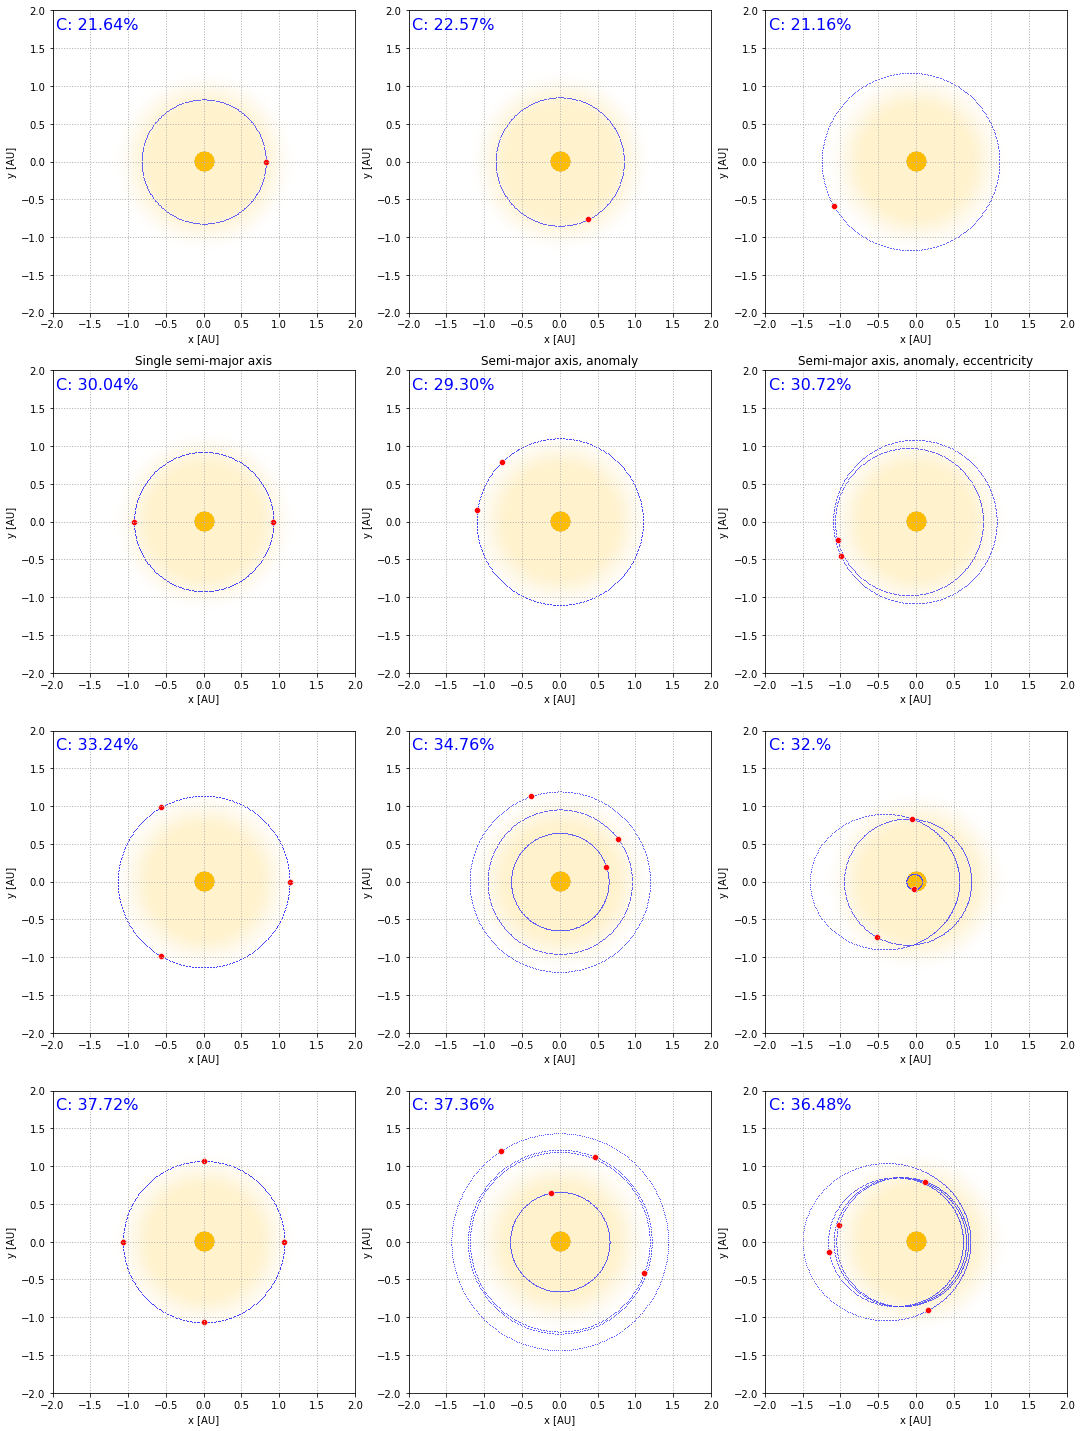
\includegraphics[width=1.0\textwidth]{img/appendix_orbit_1.png}
 \caption{Optimization solutions for 1-4 spacecraft. Left: circular co-orbital, middle: individual semi-major axis and anomaly, right: individual semi-major axis, anomaly and eccentricity.}
\end{figure}

\begin{figure}[p]
 \centering
 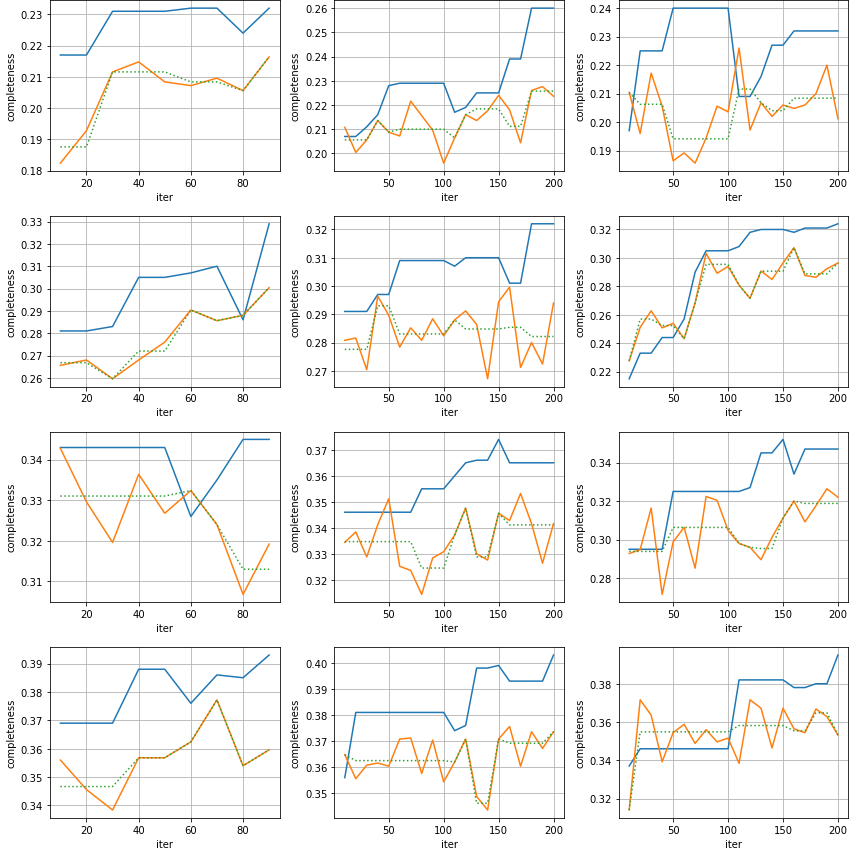
\includegraphics[width=1.0\textwidth]{img/appendix_loss_1.png}
 \caption{Learning and loss curves for optimization of 1-4 spacecraft. Blue line: learning, orange line: validation, green dotted line: average of validation for a given solution.}
\end{figure}



\begin{figure}[p]
 \centering
 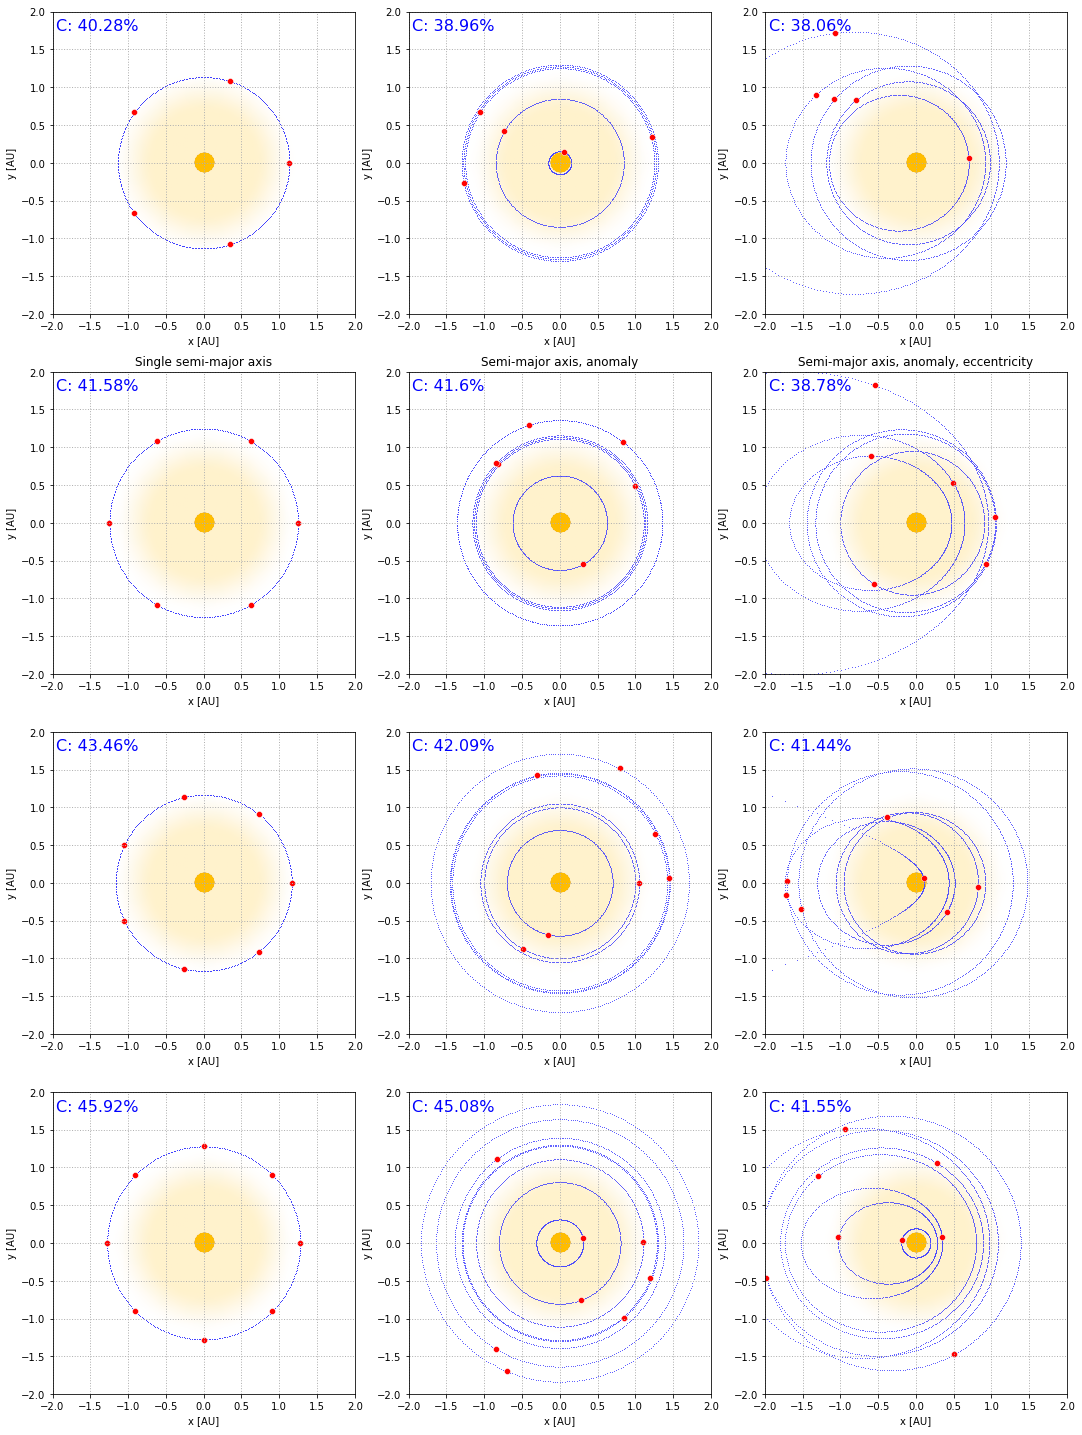
\includegraphics[width=1.0\textwidth]{img/appendix_orbit_2.png}
 \caption{Optimization solutions for 5-8 spacecraft. Left: circular co-orbital, middle: individual semi-major axis and anomaly, right: individual semi-major axis, anomaly and eccentricity.}
\end{figure}

\begin{figure}[p]
 \centering
 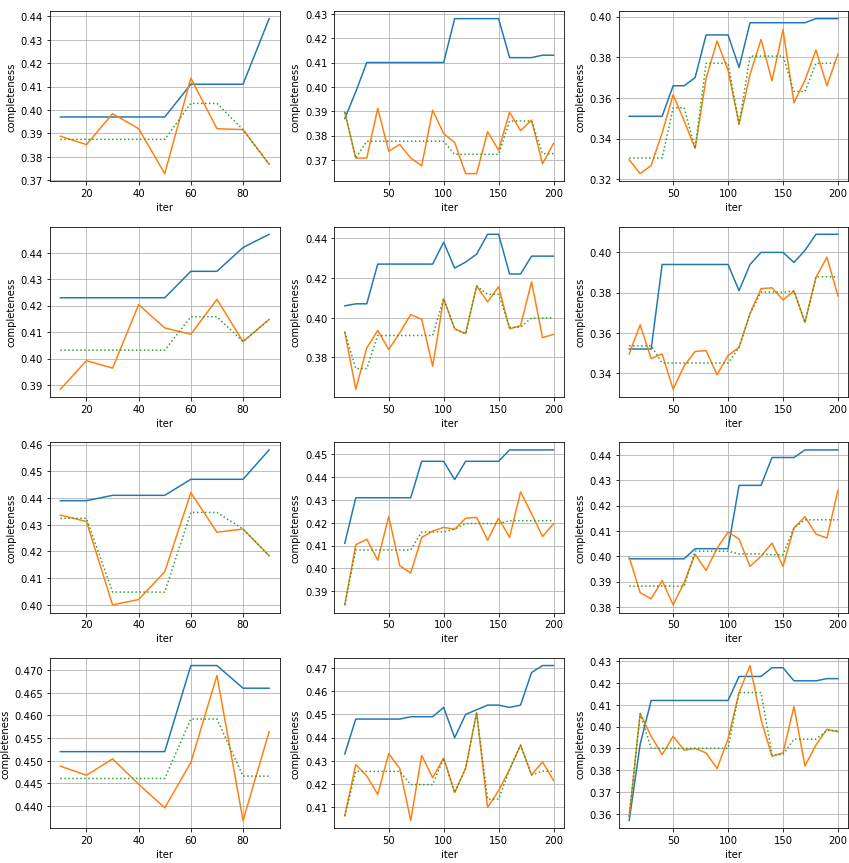
\includegraphics[width=1.0\textwidth]{img/appendix_loss_2.png}
 \caption{Learning and loss curves for optimization of 5-8 spacecraft. Blue line: learning, orange line: validation, green dotted line: average of validation for a given solution.}
\end{figure}



\begin{figure}[p]
 \centering
 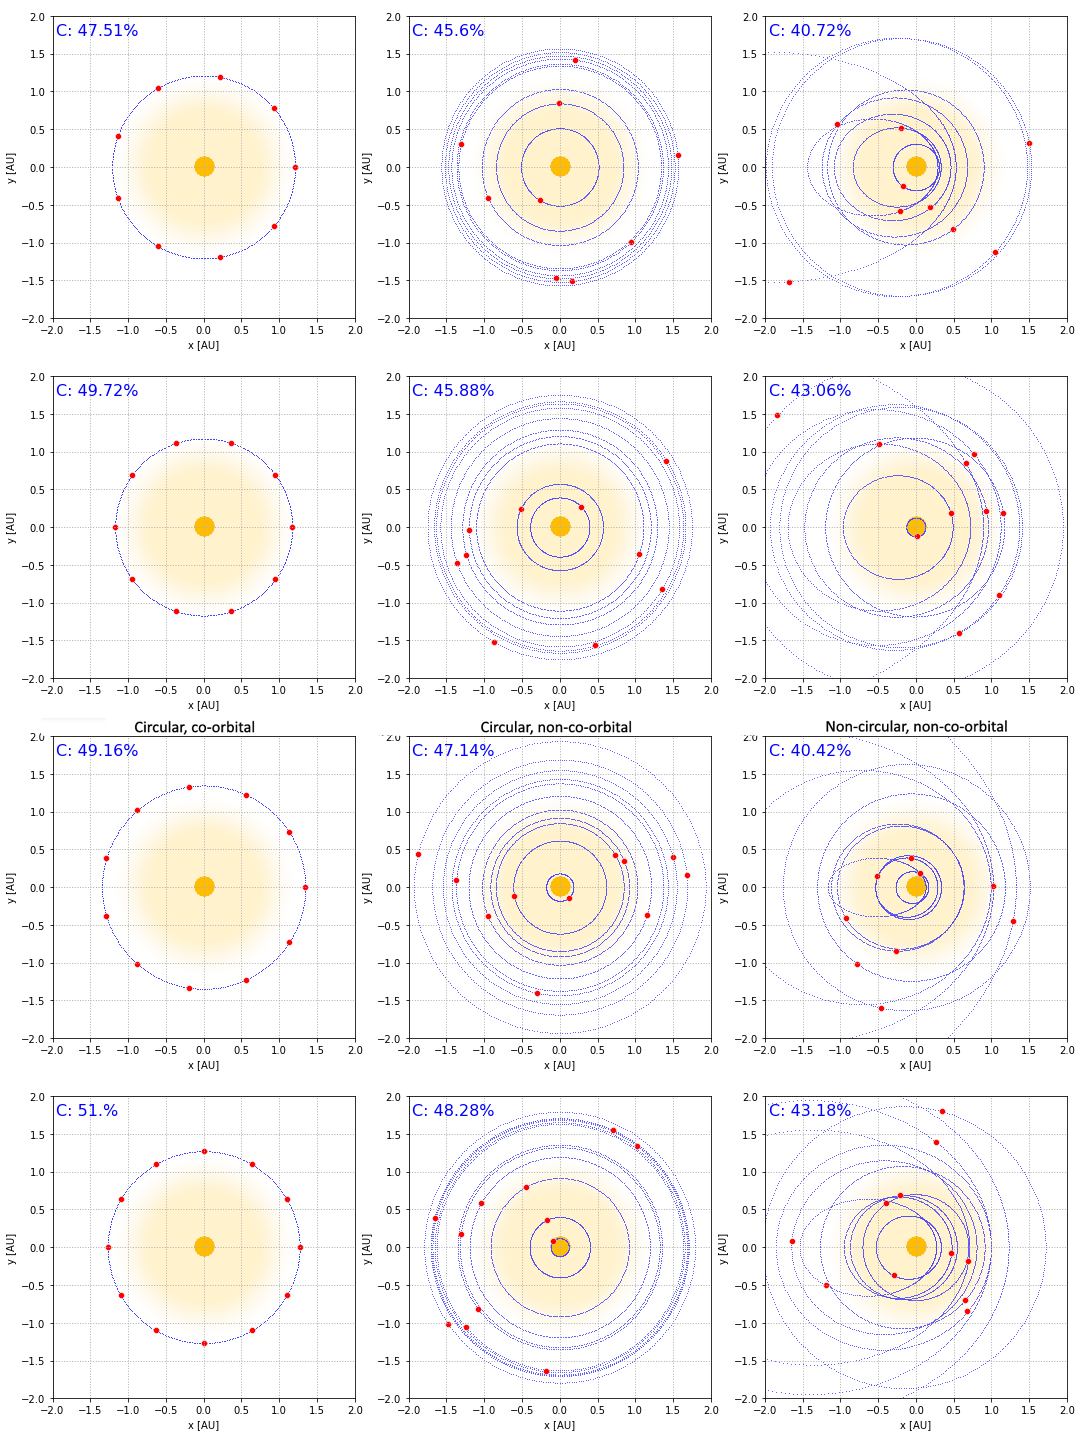
\includegraphics[width=1.0\textwidth]{img/appendix_orbit_3.png}
 \caption{Optimization solutions for 9-12 spacecraft. Left: circular co-orbital, middle: individual semi-major axis and anomaly, right: individual semi-major axis, anomaly and eccentricity.}
\end{figure}

\begin{figure}[p]
 \centering
 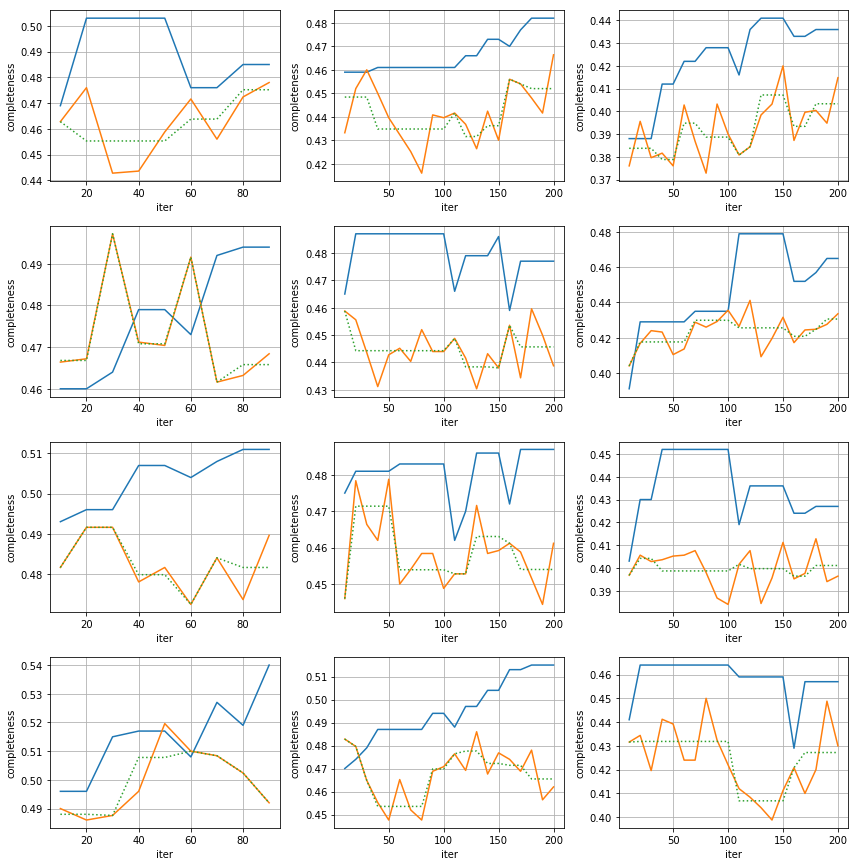
\includegraphics[width=1.0\textwidth]{img/appendix_loss_3.png}
 \caption{Learning and loss curves for optimization of 9-12 spacecraft. Blue line: learning, orange line: validation, green dotted line: average of validation for a given solution.}
\end{figure}



\begin{figure}[p]
 \centering
 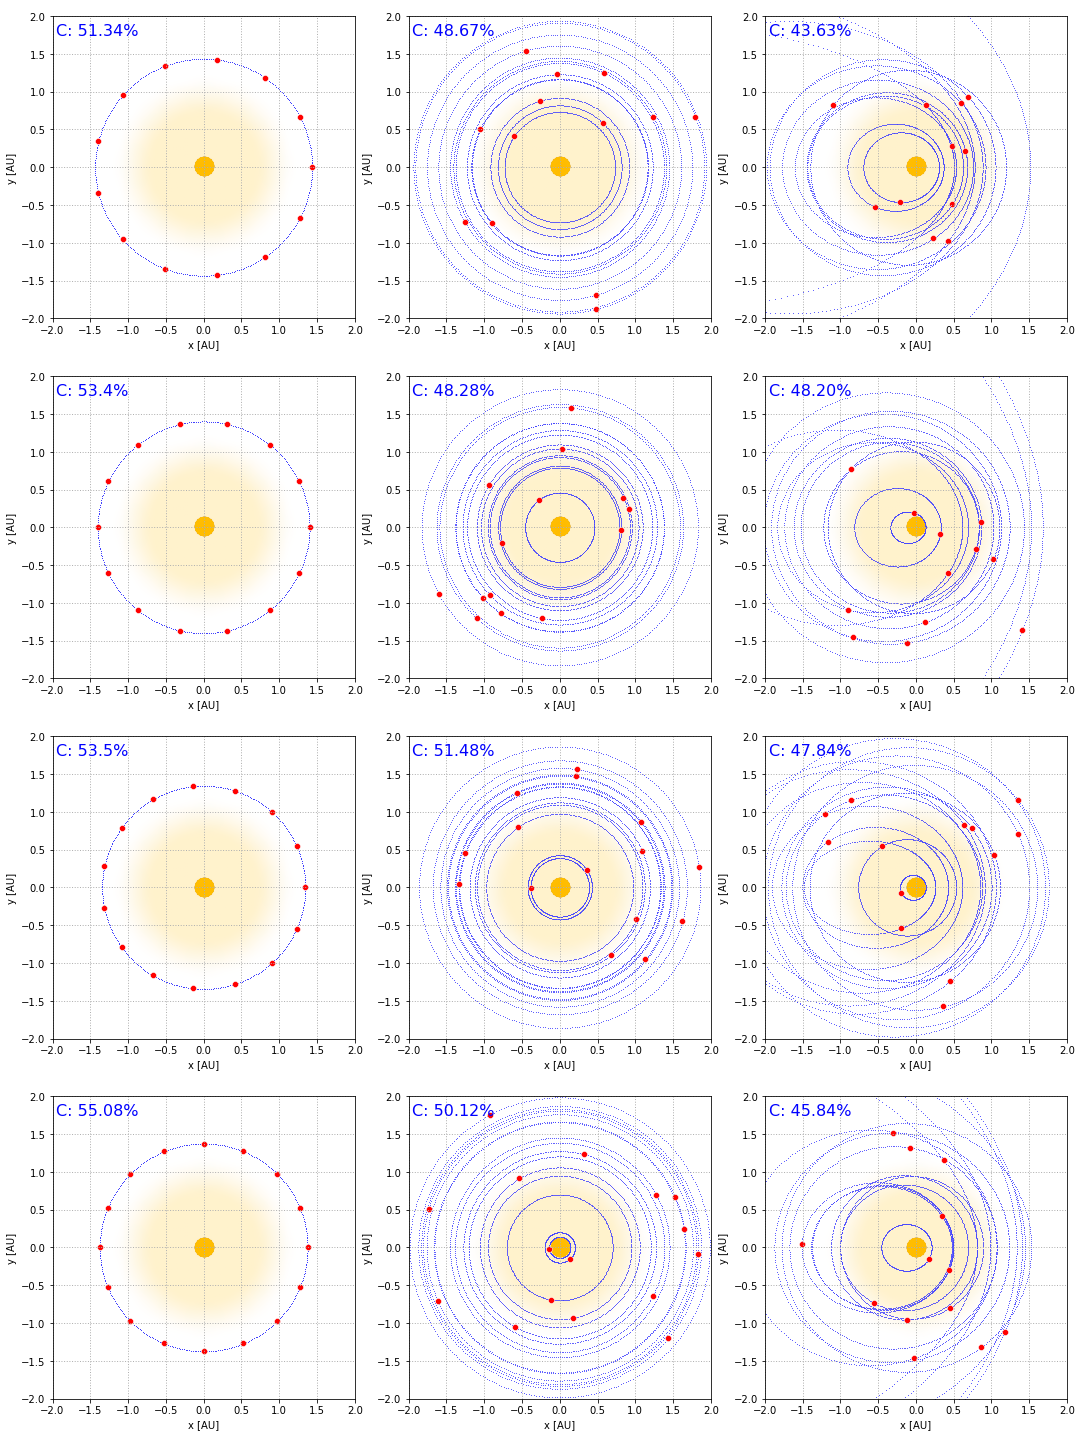
\includegraphics[width=1.0\textwidth]{img/appendix_orbit_4.png}
 \caption{Optimization solutions for 13-16 spacecraft. Left: circular co-orbital, middle: individual semi-major axis and anomaly, right: individual semi-major axis, anomaly and eccentricity.}
\end{figure}

\begin{figure}[p]
 \centering
 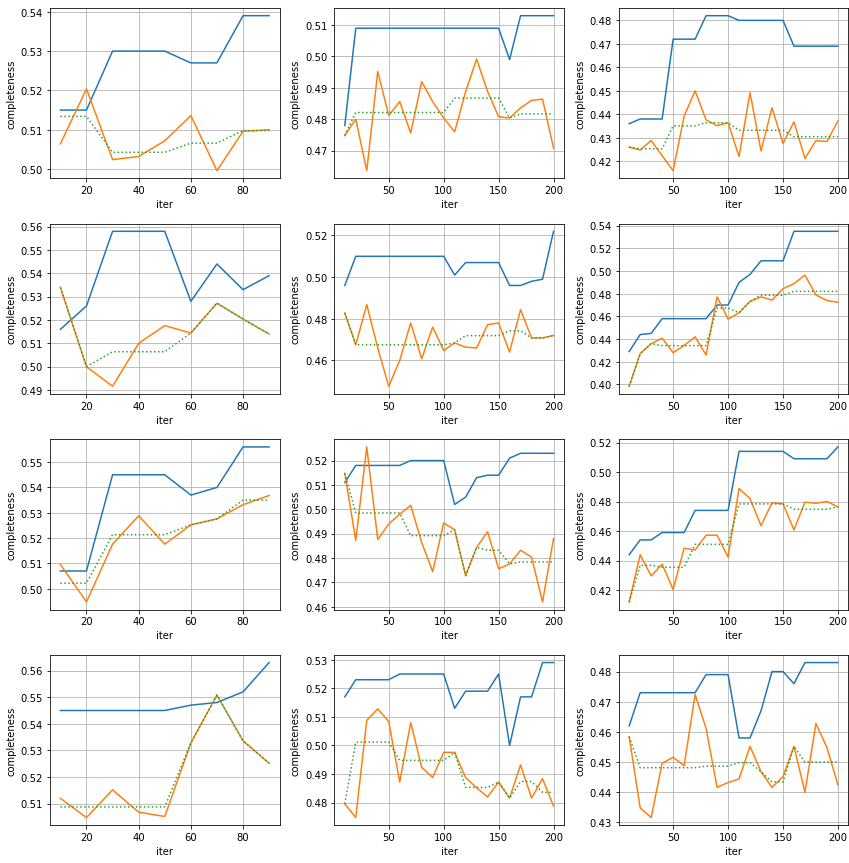
\includegraphics[width=1.0\textwidth]{img/appendix_loss_4.png}
 \caption{Learning and loss curves for optimization of 13-16 spacecraft. Blue line: learning, orange line: validation, green dotted line: average of validation for a given solution.}
\end{figure}



\begin{figure}[p]
 \centering
 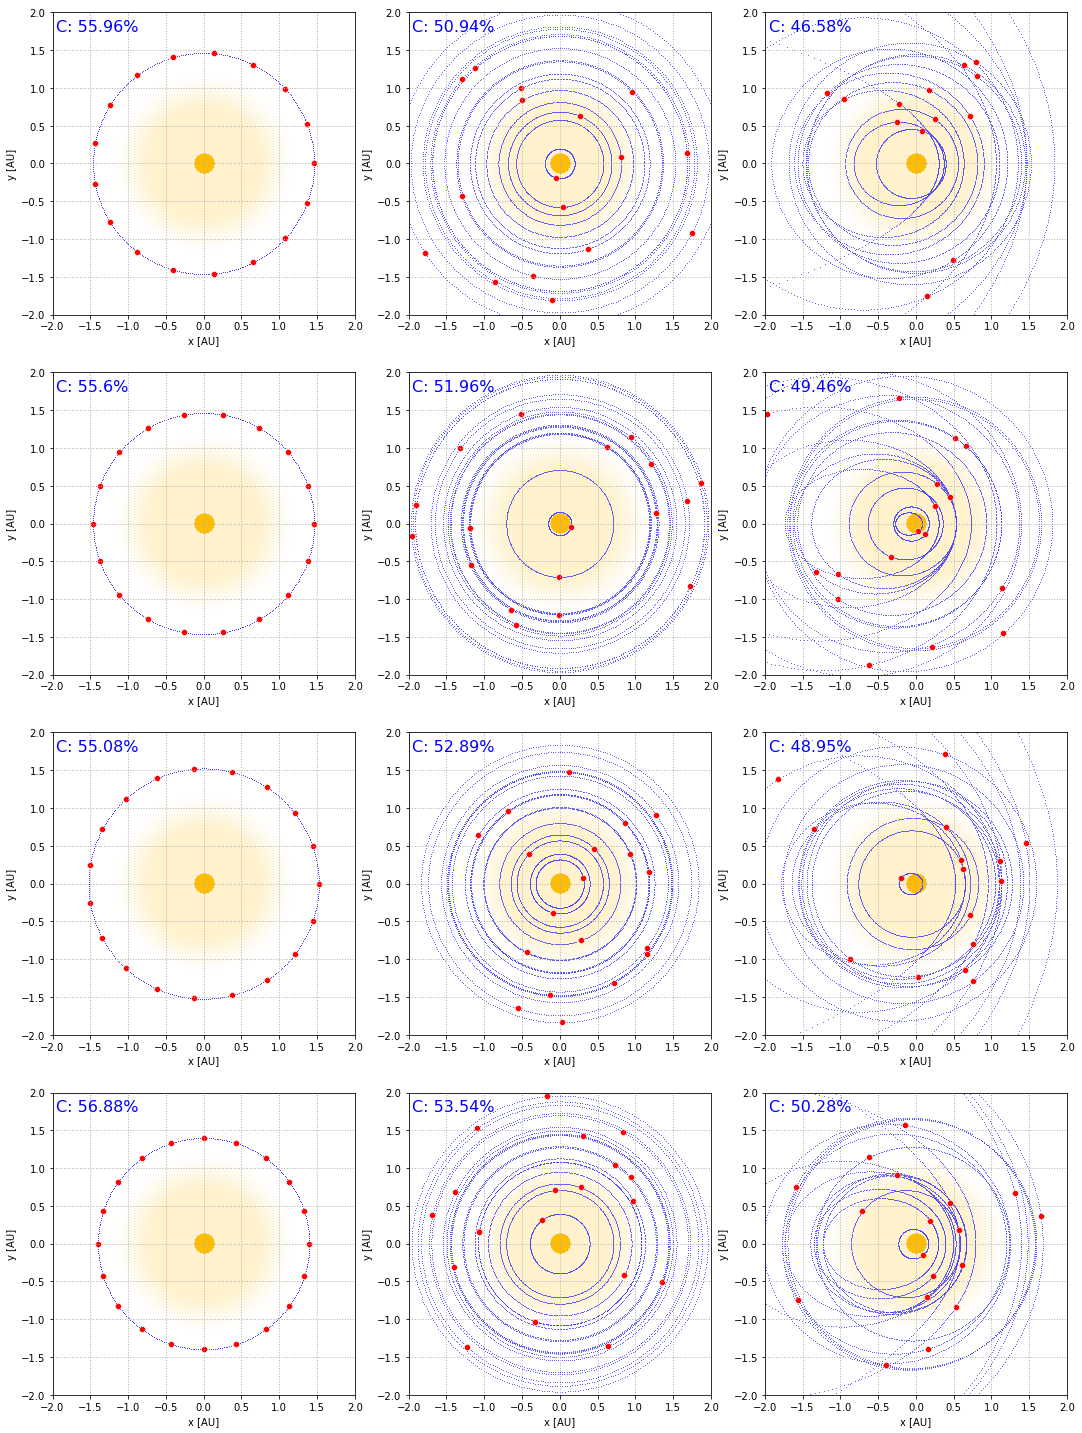
\includegraphics[width=1.0\textwidth]{img/appendix_orbit_5.png}
 \caption{Optimization solutions for 17-20 spacecraft. Left: circular co-orbital, middle: individual semi-major axis and anomaly, right: individual semi-major axis, anomaly and eccentricity.}
\end{figure}

\begin{figure}[p]
 \centering
 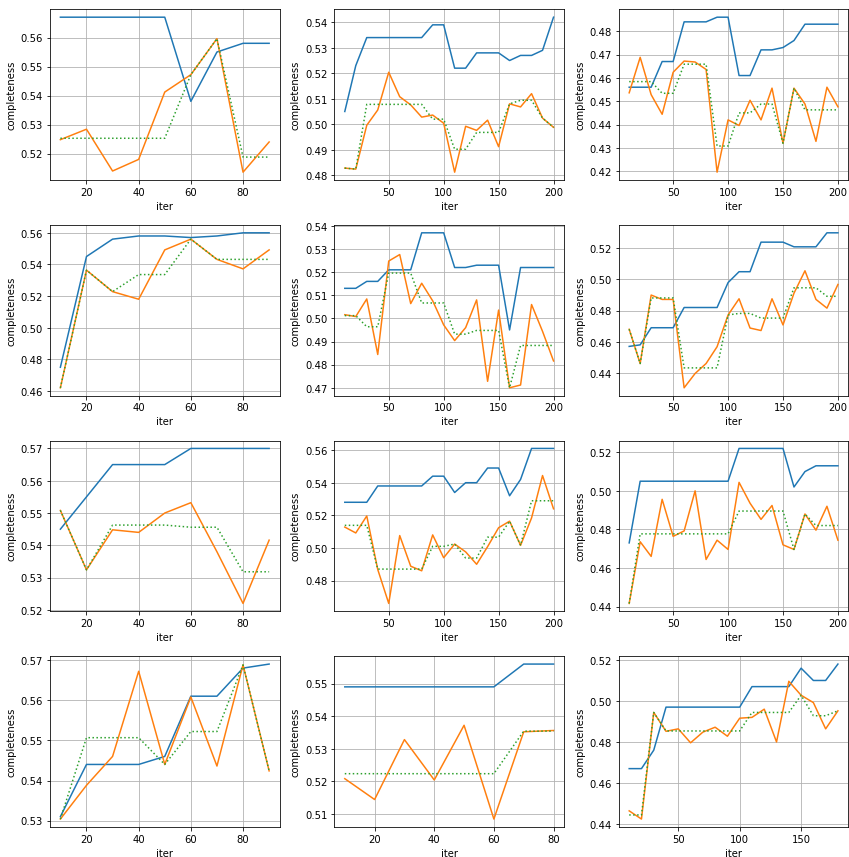
\includegraphics[width=1.0\textwidth]{img/appendix_loss_5.png}
 \caption{Learning and loss curves for optimization of 17-20 spacecraft. Blue line: learning, orange line: validation, green dotted line: average of validation for a given solution.}
\end{figure}
